%----------------------------------------------------------------------------------------
% POOLCOÖRDINATEN. Alle opgaven zijn eigen werk.
%
% Opbouw: Probleem, Start, leerstof, en op een nieuwe pagina de Opdrachten, Koppel en Test jezelf.
% Labels van dit hoofdstuk beginnen met h3-.
%----------------------------------------------------------------------------------------

\mychapter{3}{Poolcoördinaten}

\begin{probleem}
\naast{Leg twee even grote munten tegen elkaar op tafel. Hou de linkse vast en rol de rechtse er zonder glijden één keer omheen. Volg het punt $P$ van de rollende munt dat in het begin de vaste munt raakt. Welke kromme tekent $P$? Met een parametervoorstelling zoals in hoofdstuk 1 lukt het wel, maar de vergelijking in $x$ en $y$ is ingewikkeld. Bestaat er een eenvoudiger beschrijving? En hoeveel keer draait de rollende munt rond haar eigen middelpunt?}{\begin{tikzpicture}[scale=.62,font=\scriptsize]
  \draw[lijngrijs,thick,fill=black!6] (0,0) circle (1);
  \draw[accent,thick] (2,0) circle (1);
  \fill[accent] (1,0) circle (2.4pt) node[right,text=black,inner sep=2pt] {$P$};
  \draw[lijngrijs,dashed] ({1.7*cos(20)},{1.7*sin(20)}) arc[start angle=20,end angle=200,radius=1.7];
  \draw[lijngrijs,dashed,->] ({2.4*cos(40)},{2.4*sin(40)}) arc[start angle=40,end angle=110,radius=2.4];
  \node at (0,0) {vast};
\end{tikzpicture}}
\end{probleem}

\lkr{Leerplan Complementair (III-WiCo-d): LPD 10, met de drie wenken: poolcoördinaten met verwijzing naar de goniometrische vorm van complexe getallen (sectie 1), omzetten tussen pool- en cartesische vergelijkingen (sectie 2), en de bekende krommen: de spiraal van Archimedes, rozen, de cardioïde, de conchoïde van Nicomedes en de kegelsneden. Het trifolium (een roos met drie bladen) en zijn cartesische vergelijking horen bij de wenk van LPD 9. Voorkennis uit pakket 4: modulus en argument (Complexe getallen, hoofdstuk 3), de goniometrische formules (Goniometrische functies, hoofdstuk 2), de poolvergelijking van een kegelsnede (Kegelsneden, hoofdstuk 5), en hoofdstuk 1 en 2 van dit boek. De oppervlakte binnen een poolkromme hoort bij LPD 19 (Integralen in Complementair) en staat hier alleen in een Koppel-oefening.}

Een vliegtuig op een radarscherm, een komeet rond de zon, een punt op een draaiende schijf: soms is het natuurlijker om een punt vast te leggen met een afstand en een richting dan met $x$ en $y$. Je deed het al bij de complexe getallen, met de modulus en het argument, en in Kegelsneden gaf het de poolvergelijking van een kegelsnede. In dit hoofdstuk maken we er een volwaardig hulpmiddel van. Krommen die rond een punt draaien, zoals spiralen en rozen, krijgen zo een verrassend eenvoudige vergelijking. Op het einde lossen we het probleem van de twee munten op.

\begin{oefeningen}[Start]
\oef{h3-start-1}

\oef{h3-verken}
\end{oefeningen}

\lkr{Laat oefening \ref{oef:h3-verken} maken vóór de uitleg. De leerlingen tekenen een spiraal uit afstanden en hoeken, en merken dat een vergelijking in $x$ en $y$ niet zomaar te vinden is. Dat is het argument voor een vergelijking in $r$ en $\theta$.}

%========================================================================================
\section{Afstand en richting}

\subsection{Poolcoördinaten}

In de Verken-opgave lag elk punt vast door twee getallen: hoe ver het van $O$ ligt, en in welke richting. Zo werkt een radar, en zo werkt ook het vlak van Gauss: het complexe getal $z = r(\cos\theta + \mathrm{i}\sin\theta)$ ligt op afstand $r$ van 0, in de richting met argument $\theta$. Dat idee maken we los van de complexe getallen.

\begin{theorie}
\begin{minipage}[t]{.64\linewidth}
\vspace{0pt}
Kies een punt $O$, de \textbf{\textcolor{accent}{pool}}, en een halfrechte vanuit $O$, de \textbf{\textcolor{accent}{poolas}}. Een punt $P \neq O$ heeft \textbf{\textcolor{accent}{poolcoördinaten}} $[r, \theta]$ als
\begin{itemize}
\item $r = |OP|$, de afstand tot de pool;
\item $\theta$ de georiënteerde hoek van de poolas naar $[OP$.
\end{itemize}
De pool zelf is $[0, \theta]$, voor elke $\theta$.
\end{minipage}\hfill
\begin{minipage}[t]{.32\linewidth}
\vspace{1mm}
\centering
\begin{tikzpicture}[scale=.75,font=\scriptsize]
  \poolrooster{2.4}{.8}
  \draw[grijs,thick] (0,0) -- (50:2.4);
  \fill[accent] (50:2.0) circle (2.2pt) node[above left,text=black,inner sep=2pt] {$P$};
  \draw[grijs] (.6,0) arc[start angle=0,end angle=50,radius=.6];
  \node at (25:.85) {$\theta$};
  \node[above left,inner sep=1pt] at (50:1.1) {$r$};
  \node[below left,inner sep=2pt] at (0,0) {$O$};
\end{tikzpicture}
\end{minipage}
\end{theorie}

Voor de hoek gebruiken we radialen. Leg je de pool in de oorsprong en de poolas langs de positieve $x$-as, dan horen bij elk punt zowel cartesische coördinaten $(x, y)$ als poolcoördinaten $[r, \theta]$. We schrijven die laatste met vierkante haken, om ze niet te verwarren. Hoe reken je de ene om naar de andere?

\begin{theorie}
\begin{stelling}{Omzetten}
Het punt met poolcoördinaten $[r, \theta]$ heeft cartesische coördinaten

\vspace{1mm}
\qquad $\formule{x = r\cos\theta, \quad y = r\sin\theta}$

\vspace{1mm}
Omgekeerd is \quad $\formule{r = \sqrt{x^2 + y^2}}$ \quad en \quad $\formule{\tan\theta = \dfrac yx}$ \quad (als $x \neq 0$), met $\theta$ in het kwadrant van $(x, y)$.
\end{stelling}

\begin{bewijs}
Het punt $Q = \tfrac1r P$ ligt op de eenheidscirkel, op de halfrechte $[OP$, dus $Q = (\cos\theta, \sin\theta)$ en $P = rQ$. Omgekeerd is $r = |OP|$ de afstand tot de oorsprong, en $\tfrac yx = \tfrac{r\sin\theta}{r\cos\theta} = \tan\theta$.
\end{bewijs}
\end{theorie}

Pas op met de hoek: $\tan\theta = \tfrac yx$ heeft twee oplossingen tussen $0$ en $2\pi$, in tegenoverliggende kwadranten. Kijk dus altijd naar de tekens van $x$ en $y$, net zoals bij het argument van een complex getal.

\voorbeeld{}{Geef de cartesische coördinaten van het punt $P$ met poolcoördinaten $\bigl[4, \tfrac{2\pi}{3}\bigr]$.\label{vb:h3-naarcart}}{%
\uitleg{Vul in in de formules: de cosinus en sinus van $\tfrac{2\pi}{3} = 120^\circ$ ken je van de eenheidscirkel.}
\begin{stappen}
x = 4\cos\tfrac{2\pi}{3} = 4 \cdot \bigl(-\tfrac12\bigr) = -2 & In het tweede kwadrant is de cosinus negatief. \\[1ex]
y = 4\sin\tfrac{2\pi}{3} = 4 \cdot \tfrac{\sqrt3}{2} = 2\sqrt3 & Het punt $P(-2,\ 2\sqrt3)$.
\end{stappen}}

\voorbeeld{}{Geef poolcoördinaten van het punt $(-3,\ -3\sqrt3)$.\label{vb:h3-naarpool}}{%
\uitleg{Eerst de afstand, dan de hoek. Het punt ligt in het derde kwadrant: daar moet ook $\theta$ liggen.}
\naast{\begin{stappenvrij}{5.4cm}{4.6cm}
r = \sqrt{9 + 27} = 6 & De afstand tot de pool. \\[1ex]
\tan\theta = \dfrac{-3\sqrt3}{-3} = \sqrt3 & Dat geeft $\tfrac{\pi}{3}$ of $\tfrac{4\pi}{3}$. \\[2ex]
\theta = \dfrac{4\pi}{3} & Het derde kwadrant: $x$ en $y$ zijn negatief. \\[2ex]
\bigl[6, \tfrac{4\pi}{3}\bigr] & Of ook $\bigl[6, -\tfrac{2\pi}{3}\bigr]$.
\end{stappenvrij}}{\begin{tikzpicture}[scale=.36,font=\scriptsize]
  \rooster{-6}{2}{2}{-6}{2}{2}
  \draw[grijs,thick] (0,0) -- (-3,-5.196);
  \fill[accent] (-3,-5.196) circle (4pt) node[left,text=black,inner sep=2pt] {$P$};
  \draw[grijs] (1.2,0) arc[start angle=0,end angle=240,radius=1.2];
\end{tikzpicture}}}

\begin{werkwijze}
Van pool naar cartesisch: $x = r\cos\theta$ en $y = r\sin\theta$. Van cartesisch naar pool: $r = \sqrt{x^2 + y^2}$, en zoek $\theta$ met $\tan\theta = \tfrac yx$ in het kwadrant van het punt. Ligt het punt op een as, lees $\theta$ dan meteen af: $0$, $\tfrac{\pi}{2}$, $\pi$ of $\tfrac{3\pi}{2}$.
\end{werkwijze}

\nujij{Zet om: $\bigl[2, \tfrac{5\pi}{4}\bigr]$ naar cartesisch, en $(\sqrt3, -1)$ naar pool.}{$(-\sqrt2, -\sqrt2)$; en $\bigl[2, \tfrac{11\pi}{6}\bigr]$.}

\begin{oefeningen}
\oef{h3-omzet}
\end{oefeningen}

\subsection{Meer dan één naam}

Een punt heeft één paar cartesische coördinaten, maar veel paren poolcoördinaten: $\bigl[2, \tfrac{\pi}{4}\bigr]$, $\bigl[2, \tfrac{9\pi}{4}\bigr]$ en $\bigl[2, -\tfrac{7\pi}{4}\bigr]$ zijn hetzelfde punt, want je mag er telkens een volle toer bij doen. Voor de krommen verderop spreken we nog iets af: wat betekent een negatieve $r$?

\begin{theorie}
Is $r < 0$, dan is $[r, \theta]$ het punt $\bigl[|r|, \theta + \pi\bigr]$: je stapt $|r|$ af in de tegengestelde richting.
\end{theorie}

\figuren{\begin{tikzpicture}[scale=.72,font=\scriptsize]
  \poolrooster{2.4}{.8}
  \draw[grijs] (0,0) -- (30:2.4) (0,0) -- (210:2.4);
  \fill[accent] (30:1.6) circle (2.2pt) node[above left,text=black,inner sep=2pt] {$\bigl[2, \tfrac{\pi}{6}\bigr]$};
  \fill[fel!80!black] (210:1.6) circle (2.2pt) node[below right,text=black,inner sep=2pt] {$\bigl[-2, \tfrac{\pi}{6}\bigr] = \bigl[2, \tfrac{7\pi}{6}\bigr]$};
\end{tikzpicture}}

De formules $x = r\cos\theta$ en $y = r\sin\theta$ blijven gelden voor een negatieve $r$, want $\cos(\theta + \pi) = -\cos\theta$ en $\sin(\theta + \pi) = -\sin\theta$. Zo is $\bigl[-2, \tfrac{\pi}{6}\bigr]$ het punt $(-\sqrt3, -1)$.

\begin{oefeningen}
\oef{h3-namen}
\end{oefeningen}

%========================================================================================
\section{Poolvergelijkingen}

\subsection{Een kromme met \texorpdfstring{$r = f(\theta)$}{r = f(θ)}}

Een vergelijking in $x$ en $y$ beschrijft een kromme: alle punten waarvan de coördinaten aan de vergelijking voldoen. Hetzelfde kan met $r$ en $\theta$. De eenvoudigste: $r = 3$ zijn de punten op afstand 3 van de pool, een cirkel, en $\theta = \tfrac{\pi}{4}$ zijn de punten in de richting $\tfrac{\pi}{4}$, met een negatieve $r$ ook die in de tegengestelde richting: de rechte $y = x$.

\begin{theorie}
Een \textbf{\textcolor{accent}{poolvergelijking}} $\formule{r = f(\theta)}$ beschrijft de kromme van alle punten $\bigl[f(\theta), \theta\bigr]$, met $\theta$ in het domein van $f$.
\end{theorie}

Een punt ligt op de kromme als \textit{een} van zijn paren poolcoördinaten aan de vergelijking voldoet. De pool $[0, \theta]$ ligt erop als $f(\theta) = 0$ voor een of andere $\theta$. Tekenen gaat met een tabel, net zoals in hoofdstuk 1: in feite is $x = f(\theta)\cos\theta$, $y = f(\theta)\sin\theta$ een parametervoorstelling met parameter $\theta$.

\voorbeeld{}{Teken de kromme $r = 4\cos\theta$ voor $\theta \in [0, \pi]$.\label{vb:h3-tekenen}}{%
\uitleg{Een tabel met $\theta$ en $r$. Zet elk punt op afstand $r$ in de richting $\theta$, en bij een negatieve $r$ in de tegengestelde richting.}
\naast{{\small\renewcommand{\arraystretch}{1.35}%
\begin{tabular}{|c|c|c|c|c|c|c|c|}
\hline
$\theta$ & $0$ & $\tfrac{\pi}{6}$ & $\tfrac{\pi}{3}$ & $\tfrac{\pi}{2}$ & $\tfrac{2\pi}{3}$ & $\tfrac{5\pi}{6}$ & $\pi$ \\ \hline
$r$ & $4$ & $3{,}46$ & $2$ & $0$ & $-2$ & $-3{,}46$ & $-4$ \\ \hline
\end{tabular}}

\medskip
Voor $\theta \in \bigl[0, \tfrac{\pi}{2}\bigr]$ loopt het punt van $(4, 0)$ naar de pool, boven de poolas. Daarna is $r$ negatief: $\bigl[-2, \tfrac{2\pi}{3}\bigr] = \bigl[2, \tfrac{5\pi}{3}\bigr]$ ligt onder de poolas. Bij $\theta = \pi$ is het punt weer $(4, 0)$. De kromme lijkt een cirkel door de pool, één keer doorlopen.}{\begin{tikzpicture}[scale=.6,font=\scriptsize]
  \poolrooster{4}{1}
  \poolkromme{0}{180}{4*cos(\t)}
  \foreach \h in {0,30,...,180}{\fill[accent] ({4*cos(\h)*cos(\h)},{4*cos(\h)*sin(\h)}) circle (2pt);}
  \node[below right,inner sep=1pt] at (4,0) {$4$};
  \fill[fel!80!black] (120:-2) circle (2.4pt) node[below,text=black,inner sep=3pt] {$\theta = \tfrac{2\pi}{3}$};
\end{tikzpicture}}}

\begin{werkwijze}
Maak een tabel van $\theta$ en $r$, met de hoeken van de eenheidscirkel. Teken een poolrooster: cirkels rond de pool en halfrechten per hoek. Zet elk punt op afstand $|r|$ in de richting $\theta$, of in de richting $\theta + \pi$ als $r < 0$. Verbind in de volgorde van $\theta$.
\end{werkwijze}

\nujij{Teken $r = 2\sin\theta$ voor $\theta \in [0, \pi]$.}{Een cirkel door de pool boven de poolas, met middelpunt $(0, 1)$ en straal 1.}

\begin{oefeningen}
\oef{h3-tekenen}
\end{oefeningen}

\subsection{Omzetten}

Is $r = 4\cos\theta$ echt een cirkel? Dat bewijs je door de poolvergelijking om te zetten naar een cartesische vergelijking. Daarvoor heb je drie verbanden nodig: $r\cos\theta = x$, $r\sin\theta = y$ en $r^2 = x^2 + y^2$. Vaak moet je eerst met $r$ vermenigvuldigen om die vormen te krijgen. Zo wordt $r = 4\cos\theta$ eerst $r^2 = 4r\cos\theta$, en dan $x^2 + y^2 = 4x$, of $(x - 2)^2 + y^2 = 4$: een cirkel met middelpunt $(2, 0)$ en straal 2.

\voorbeeld{}{Welke kromme is $r = \dfrac{2}{1 - \cos\theta}$?\label{vb:h3-naarcartvgl}}{%
\uitleg{Dat lijkt op de poolvergelijking van een kegelsnede uit Kegelsneden, met $e = 1$ en een minteken: een parabool met de richtlijn links van de pool. We controleren het door om te zetten.}
\naast{\begin{stappenvrij}{5.4cm}{4.4cm}
r - r\cos\theta = 2 & Vermenigvuldig met de noemer. \\[1ex]
\sqrt{x^2 + y^2} = 2 + x & $r = \sqrt{x^2 + y^2}$ en $r\cos\theta = x$. \\[1ex]
x^2 + y^2 = 4 + 4x + x^2 & Kwadrateren; het rechterlid is $r \geqslant 0$. \\[1ex]
y^2 = 4x + 4 & Een parabool met top $(-1, 0)$ en brandpunt in de pool.
\end{stappenvrij}}{\begin{tikzpicture}[scale=.42,font=\scriptsize]
  \rooster{-2}{1}{4}{-4}{1}{4}
  \begin{scope}\clip (-2,-4.3) rectangle (4.3,4.3);
  \poolkromme{38}{322}{2/(1-cos(\t))}
  \end{scope}
  \fill (0,0) circle (3pt);
\end{tikzpicture}}}

Andersom gaat het meestal eenvoudiger: vervang $x$ door $r\cos\theta$ en $y$ door $r\sin\theta$, en los op naar $r$. Een ingewikkelde cartesische vergelijking wordt zo soms heel kort.

\voorbeeld{}{Geef een poolvergelijking van de lemniscaat $(x^2 + y^2)^2 = 2(x^2 - y^2)$ uit hoofdstuk 2.\label{vb:h3-naarpoolvgl}}{%
\uitleg{Vervang $x^2 + y^2$ door $r^2$, en $x^2 - y^2$ door $r^2(\cos^2\theta - \sin^2\theta)$.}
\naast{\begin{stappenvrij}{5.4cm}{4.4cm}
r^4 = 2r^2(\cos^2\theta - \sin^2\theta) & Invullen. \\[1ex]
r^4 = 2r^2\cos2\theta & De verdubbelingsformule. \\[1ex]
r^2 = 2\cos2\theta & Deel door $r^2$; de pool ligt er ook op, bij $\theta = \tfrac{\pi}{4}$.
\end{stappenvrij}}{\begin{tikzpicture}[scale=.85,font=\scriptsize]
  \poolrooster{1.6}{.5}
  \pkromme{0}{360}{1.41421*cos(\t)/(1+sin(\t)^2)}{1.41421*sin(\t)*cos(\t)/(1+sin(\t)^2)}
\end{tikzpicture}}
Lees de poolvergelijking: een punt bestaat alleen als $\cos2\theta \geqslant 0$, dus voor $\theta \in \bigl[-\tfrac{\pi}{4}, \tfrac{\pi}{4}\bigr]$ en $\bigl[\tfrac{3\pi}{4}, \tfrac{5\pi}{4}\bigr]$. Het verste punt ligt bij $\theta = 0$, op afstand $\sqrt2$. Dat is veel duidelijker dan in de cartesische vergelijking.}

\begin{werkwijze}
Van pool naar cartesisch: vermenigvuldig zo nodig met $r$ of met een noemer, en vervang $r\cos\theta$ door $x$, $r\sin\theta$ door $y$ en $r^2$ door $x^2 + y^2$. Van cartesisch naar pool: vervang $x$ en $y$ door $r\cos\theta$ en $r\sin\theta$, vereenvoudig met de goniometrische formules, en los op naar $r$. Let op of de pool verloren gaat of erbij komt als je door $r$ deelt.
\end{werkwijze}

\nujij{Zet om: $x^2 + y^2 = 6y$ naar pool, en $r = \dfrac{3}{\cos\theta}$ naar cartesisch.}{$r^2 = 6r\sin\theta$, dus $r = 6\sin\theta$; en $r\cos\theta = 3$, de rechte $x = 3$.}

\begin{oefeningen}
\oef{h3-naarcart}

\oef{h3-naarpool}
\end{oefeningen}

%========================================================================================
\section{Spiralen en rozen}

\subsection{De spiraal van Archimedes}

Een mier wandelt met constante snelheid van het midden naar de rand van een draaiende grammofoonplaat. Haar afstand tot het midden groeit evenredig met de tijd, en dus ook met de hoek waarover de plaat gedraaid is. In poolcoördinaten is dat eenvoudig: $r$ is evenredig met $\theta$. Archimedes schreef rond 225 voor Christus een heel boek over die kromme, zonder coördinaten.

\begin{theorie}
De \textbf{\textcolor{accent}{spiraal van Archimedes}} is de kromme $\formule{r = a\theta}$ met $a > 0$ en $\theta \geqslant 0$.

\begin{stelling}{Gelijke afstanden}
Op elke halfrechte vanuit de pool liggen opeenvolgende windingen van de spiraal van Archimedes op dezelfde afstand $\formule{2\pi a}$ van elkaar.
\end{stelling}

\begin{bewijs}
Twee opeenvolgende snijpunten met dezelfde halfrechte horen bij $\theta$ en $\theta + 2\pi$. Hun afstanden tot de pool verschillen $a(\theta + 2\pi) - a\theta = 2\pi a$.
\end{bewijs}
\end{theorie}

\figuren{\begin{tikzpicture}[scale=.55,font=\scriptsize]
  \poolrooster{3.4}{1}
  \poolkromme{0}{1080}{.16*\t*pi/180}
  \draw[fel!80!black,very thick] (60:{.16*pi/3}) -- (60:{.16*7*pi/3}) -- (60:{.16*13*pi/3});
  \foreach \k in {1,7,13}{\fill[fel!80!black] (60:{.16*\k*pi/3}) circle (2pt);}
  \node[right,inner sep=3pt] at (60:{.16*10*pi/3}) {$2\pi a$};
\end{tikzpicture}}

Daarom heeft een opgerold tapijt, de groef van een grammofoonplaat of een rol papier de vorm van een spiraal van Archimedes: bij elke toer komt er dezelfde dikte bij.

\voorbeeld{}{De groef van een grammofoonplaat loopt in 20 minuten van $r = 14{,}6$~cm naar $r = 6{,}0$~cm. De plaat draait $33\tfrac13$ toeren per minuut. Hoe ver liggen twee windingen van de groef uit elkaar?\label{vb:h3-spiraal}}{%
\uitleg{De groef is een spiraal van Archimedes, naar binnen doorlopen. Tel de windingen: de afstand ertussen is overal dezelfde.}
\begin{stappen}
20 \cdot 33\tfrac13 \approx 667 & Het aantal toeren, dus het aantal windingen. \\[1ex]
\dfrac{14{,}6 - 6{,}0}{667} \approx 0{,}013 & De afstand tussen twee windingen, in cm: 0,13~mm. \\[2ex]
2\pi a = 0{,}0129 \ \Rightarrow\ a \approx 0{,}0021 & Met $r = 6 + a\theta$ wordt de groef van binnen naar buiten beschreven.
\end{stappen}}

\nujij{Hoe ver liggen de windingen van $r = 3\theta$ uit elkaar?}{$2\pi \cdot 3 = 6\pi \approx 18{,}8$.}

\begin{oefeningen}
\oef{h3-spiraal}
\end{oefeningen}

\subsection{Rozen}

Wat gebeurt er als $r$ schommelt in plaats van te groeien? Neem $r = \cos2\theta$. Terwijl $\theta$ één toer maakt, gaat $\cos2\theta$ twee keer op en neer, en elke keer dat $r$ van 0 naar een top en terug gaat, ontstaat er een blad. Zo krijg je bloemen.

\begin{theorie}
Een \textbf{\textcolor{accent}{roos}} is een kromme $\formule{r = a\cos(n\theta)}$ of $\formule{r = a\sin(n\theta)}$, met $a > 0$ en $n \geqslant 2$ een natuurlijk getal. Bij $n = 3$ heet ze een \textbf{\textcolor{accent}{trifolium}} (klaverblad).

\begin{stelling}{Aantal bladen}
De roos $r = a\cos(n\theta)$ heeft $n$ bladen als $n$ oneven is, en $2n$ bladen als $n$ even is.
\end{stelling}

\begin{bewijs}
Op $[0, 2\pi[$ is $r = 0$ bij $2n$ hoeken, die $\tfrac{\pi}{n}$ uit elkaar liggen. Tussen twee opeenvolgende nulpunten tekent $r$ één blad: $2n$ bladen, als ze verschillend zijn. Vergelijk nu $\theta$ en $\theta + \pi$: dan is $\cos\bigl(n(\theta + \pi)\bigr) = \cos(n\theta + n\pi)$.
\bewijsregel{n \text{ oneven: } r(\theta + \pi) = -r(\theta), \qquad n \text{ even: } r(\theta + \pi) = r(\theta) .}
Bij $n$ oneven is $\bigl[-r(\theta), \theta + \pi\bigr] = \bigl[r(\theta), \theta\bigr]$: het tweede halve toertje tekent dezelfde bladen opnieuw, en er zijn er $n$. Bij $n$ even is $\bigl[r(\theta), \theta + \pi\bigr]$ het tegenovergestelde punt, en zijn de $2n$ bladen verschillend.
\end{bewijs}
\end{theorie}

\figuren{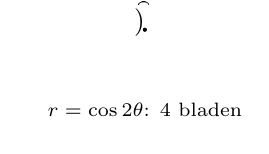
\begin{tikzpicture}[scale=.75,font=\scriptsize]
  \poolkromme{0}{360}{cos(2*\t)}
  \fill (0,0) circle (1pt);
  \node at (0,-1.35) {$r = \cos2\theta$: 4 bladen};
\end{tikzpicture}\qquad
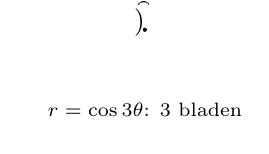
\begin{tikzpicture}[scale=.75,font=\scriptsize]
  \poolkromme{0}{180}{cos(3*\t)}
  \fill (0,0) circle (1pt);
  \node at (0,-1.35) {$r = \cos3\theta$: 3 bladen};
\end{tikzpicture}\qquad
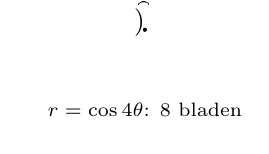
\begin{tikzpicture}[scale=.75,font=\scriptsize]
  \poolkromme{0}{360}{cos(4*\t)}
  \fill (0,0) circle (1pt);
  \node at (0,-1.35) {$r = \cos4\theta$: 8 bladen};
\end{tikzpicture}\qquad
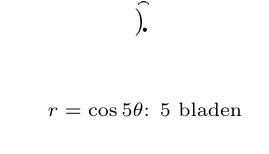
\begin{tikzpicture}[scale=.75,font=\scriptsize]
  \poolkromme{0}{180}{cos(5*\t)}
  \fill (0,0) circle (1pt);
  \node at (0,-1.35) {$r = \cos5\theta$: 5 bladen};
\end{tikzpicture}}

De bladen hebben lengte $a$, de grootste waarde van $|r|$. Bij $r = a\sin(n\theta)$ zijn het dezelfde rozen, gedraaid.

\voorbeeld{}{Geef een cartesische vergelijking van het trifolium $r = \cos3\theta$.\label{vb:h3-trifolium}}{%
\uitleg{Vermenigvuldig met $r^3$, zodat er $r^3\cos3\theta$ staat. Dat is het reële deel van $\bigl(r(\cos\theta + \mathrm{i}\sin\theta)\bigr)^3 = (x + y\mathrm{i})^3$, volgens De Moivre.}
\begin{stappen}
r^4 = r^3\cos3\theta & Vermenigvuldig met $r^3$. \\[1ex]
(x + y\mathrm{i})^3 = x^3 + 3x^2y\mathrm{i} - 3xy^2 - y^3\mathrm{i} & Het binomium van Newton, met $\mathrm{i}^2 = -1$. \\[1ex]
r^3\cos3\theta = x^3 - 3xy^2 & Het reële deel. \\[1ex]
(x^2 + y^2)^2 = x^3 - 3xy^2 & Met $r^4 = (x^2 + y^2)^2$.
\end{stappen}
Zonder complexe getallen kan het ook, met $\cos3\theta = 4\cos^3\theta - 3\cos\theta$ (opdracht~\ref{oef:h1-o22} van hoofdstuk 1). In de poolvergelijking zie je meteen de drie bladen; in de cartesische vergelijking zie je vooral dat de kromme symmetrisch is ten opzichte van de $x$-as.}

\begin{werkwijze}
Om een roos te tekenen: zoek de hoeken waar $r = 0$ (de bladen beginnen en eindigen daar) en waar $|r| = a$ (de toppen). Tel de bladen met de stelling, en teken ze gelijkmatig verdeeld rond de pool.
\end{werkwijze}

\nujij{Hoeveel bladen heeft $r = 3\sin4\theta$, en hoe lang zijn ze?}{8 bladen van lengte 3.}

\begin{oefeningen}
\oef{h3-roos}
\end{oefeningen}

%========================================================================================
\section{Krommen uit een constructie}

\subsection{De conchoïde van Nicomedes}

Rond 200 voor Christus zocht Nicomedes een manier om een hoek in drie gelijke delen te verdelen. Hij gebruikte een kromme die je zo construeert: neem een punt $O$ en een rechte $l$ op afstand $a$ van $O$. Trek een rechte door $O$, die $l$ snijdt in $Q$, en zet op die rechte de twee punten op afstand $b$ van $Q$. Alle punten die je zo krijgt, vormen de \textit{conchoïde}, naar het Griekse woord voor schelp.

\begin{theorie}
\begin{minipage}[t]{.6\linewidth}
\vspace{0pt}
\begin{stelling}{Conchoïde van Nicomedes}
Met $O$ als pool en $l \leftrightarrow x = a$ heeft de conchoïde als poolvergelijking

\vspace{1mm}
\qquad $\formule{r = \dfrac{a}{\cos\theta} + b}$ \quad met $\theta \in \bigl]-\tfrac{\pi}{2}, \tfrac{\pi}{2}\bigr[ \cup \bigl]\tfrac{\pi}{2}, \tfrac{3\pi}{2}\bigr[$.
\end{stelling}

\begin{bewijs}
De halfrechte met hoek $\theta \in \bigl]-\tfrac{\pi}{2}, \tfrac{\pi}{2}\bigr[$ snijdt $l$ in $Q$ met $r\cos\theta = a$, dus $Q = \bigl[\tfrac{a}{\cos\theta}, \theta\bigr]$. De twee punten op afstand $b$ zijn $\bigl[\tfrac{a}{\cos\theta} + b, \theta\bigr]$ en $\bigl[\tfrac{a}{\cos\theta} - b, \theta\bigr]$. Het tweede is ook $\bigl[\tfrac{a}{\cos(\theta + \pi)} + b, \theta + \pi\bigr]$, want $\cos(\theta + \pi) = -\cos\theta$, en dat hoort bij de hoeken in $\bigl]\tfrac{\pi}{2}, \tfrac{3\pi}{2}\bigr[$.
\end{bewijs}
\end{minipage}\hfill
\begin{minipage}[t]{.36\linewidth}
\vspace{2mm}
\centering
\begin{tikzpicture}[scale=.62,font=\scriptsize]
  \draw[->,lijngrijs] (-1.6,0) -- (4.6,0);
  \draw[grijs,thick] (1,-3) -- (1,3) node[below right,text=black] {$l$};
  \begin{scope}\clip (-1.6,-3) rectangle (4.4,3);
  \poolkromme{-75}{75}{1/cos(\t)+2}
  \poolkromme{97}{263}{1/cos(\t)+2}
  \end{scope}
  \draw[grijs] (0,0) -- (35:3.8);
  \fill (0,0) circle (1.6pt) node[below left,inner sep=1pt] {$O$};
  \fill (35:1.221) circle (1.6pt) node[below right,inner sep=1pt] {$Q$};
  \fill[accent] (35:3.221) circle (2pt);
  \draw[fel!80!black,very thick] (35:1.221) -- node[above left,text=black,inner sep=1pt] {$b$} (35:3.221);
  \node[below,inner sep=2pt] at (.5,0) {$a$};
\end{tikzpicture}
\end{minipage}
\end{theorie}

De kromme heeft twee takken: de buitenste, aan de andere kant van $l$, en de binnenste, bij $O$. Beide naderen $l$ als $\theta$ naar $\pm\tfrac{\pi}{2}$ gaat: $l$ is een asymptoot. Is $b > a$, dan maakt de binnenste tak een lus door $O$, zoals in de figuur. In opdracht~\ref{oef:h3-o19} zie je hoe Nicomedes er een hoek mee in drie deelde.

\voorbeeld{}{Neem de conchoïde met $a = 1$ en $b = 2$. Bereken de punten bij $\theta = 0$ en $\theta = \pi$, en zoek waar de kromme door de pool gaat.\label{vb:h3-conchoide}}{%
\uitleg{Vul in in $r = \tfrac{1}{\cos\theta} + 2$. De pool hoort erbij als $r = 0$.}
\begin{stappen}
r(0) = 1 + 2 = 3 & Het punt $(3, 0)$ op de buitenste tak. \\[1ex]
r(\pi) = -1 + 2 = 1 & $[1, \pi]$, het punt $(-1, 0)$ op de lus. \\[1ex]
\tfrac{1}{\cos\theta} = -2 \ \Rightarrow\ \theta = \tfrac{2\pi}{3} \text{ of } \tfrac{4\pi}{3} & Twee keer door de pool: de lus begint en eindigt daar.
\end{stappen}}

\begin{oefeningen}
\oef{h3-conch}
\end{oefeningen}

\subsection{De cardioïde}

Terug naar de munten. Noem de straal $a$, leg het middelpunt van de vaste munt in de oorsprong, en laat de rollende munt vertrekken met haar middelpunt in $(2a, 0)$, zodat $P$ in $A(a, 0)$ ligt. Zoals bij de cycloïde volgen we het middelpunt en draaien we rond het middelpunt.

Het middelpunt $M$ van de rollende munt blijft op afstand $2a$ van $O$: $M = (2a\cos t, 2a\sin t)$, met $t$ de hoek van $\overrightarrow{OM}$. De munt rolt zonder glijden: de boog die ze aflegt over de vaste munt, $at$, is ook de boog op haar eigen rand tussen $P$ en het raakpunt. Daardoor is de straal $\overrightarrow{MP}$ over een hoek $2t$ gedraaid ten opzichte van het begin: $t$ omdat $M$ rond $O$ draait, en nog eens $t$ door het rollen. Zo krijg je de parametervoorstelling
\[ x = 2a\cos t - a\cos2t, \qquad y = 2a\sin t - a\sin2t . \]
Kijk nu vanuit het beginpunt $A$, en leg daar de pool.

\begin{theorie}
\begin{stelling}{Cardioïde}
Met $A(a, 0)$ als pool beschrijft $P$ de kromme \qquad $\formule{r = 2a(1 - \cos\theta)}$

\vspace{1mm}
en de hoek $\theta$ is de hoek $t$ van $\overrightarrow{OM}$. Die kromme heet een \textbf{\textcolor{accent}{cardioïde}} of hartlijn.
\end{stelling}

\begin{bewijs}
Met $\cos2t = 2\cos^2t - 1$ en $\sin2t = 2\sin t\cos t$ is
\bewijsregel{\overrightarrow{AP} = \bigl(2a\cos t - 2a\cos^2t,\ 2a\sin t - 2a\sin t\cos t\bigr) = 2a(1 - \cos t)\,(\cos t,\ \sin t) .}
Het punt $P$ ligt dus vanuit $A$ in de richting $t$, op afstand $2a(1 - \cos t) \geqslant 0$.
\end{bewijs}
\end{theorie}

\figuren{\begin{tikzpicture}[scale=.75,font=\scriptsize]
  \draw[->,lijngrijs] (-3.6,0) -- (2.6,0) node[right,text=black] {$x$};
  \draw[->,lijngrijs] (0,-2.4) -- (0,2.9) node[above,text=black] {$y$};
  \draw[lijngrijs,thick,fill=black!6] (0,0) circle (1);
  \pkromme{0}{360}{2*cos(\t)-cos(2*\t)}{2*sin(\t)-sin(2*\t)}
  \draw[grijs] (0,0) -- ({2*cos(110)},{2*sin(110)});
  \draw[lijngrijs] ({2*cos(110)},{2*sin(110)}) circle (1);
  \fill ({2*cos(110)},{2*sin(110)}) circle (1.4pt) node[above,inner sep=2pt] {$M$};
  \fill (1,0) circle (1.6pt) node[below right,inner sep=1pt] {$A$};
  \fill[accent] ({2*cos(110)-cos(220)},{2*sin(110)-sin(220)}) circle (2pt) node[right,text=black,inner sep=2pt] {$P$};
  \draw[fel!80!black,thick] (1,0) -- ({2*cos(110)-cos(220)},{2*sin(110)-sin(220)});
  \node[fel!80!black] at (.95,.75) {$r$};
  \node at (0,-.55) {$O$};
\end{tikzpicture}}

Het hart ligt op zijn zij: de spits ligt in $A$, waar $r = 0$, en het verste punt ligt bij $\theta = \pi$, op afstand $4a$. Elke kromme $r = c(1 \pm \cos\theta)$ of $r = c(1 \pm \sin\theta)$ is een gedraaide cardioïde.

\subsection{Terug naar het probleem}

\voorbeeld{}{Twee munten met straal $a = 1$~cm. Welke kromme beschrijft $P$? Hoe ver komt $P$ van zijn beginpunt? En hoe vaak draait de rollende munt rond haar middelpunt?\label{vb:h3-terug}}{%
\uitleg{De stelling geeft de kromme. Voor het aantal draaiingen kijk je naar de hoek van $\overrightarrow{MP}$.}
\naast{\begin{stappenvrij}{4.6cm}{4.6cm}
r = 2(1 - \cos\theta) & Een cardioïde, met de pool in het beginpunt $A$. \\[1ex]
r(\pi) = 4 & Het verste punt: 4~cm, als de rollende munt aan de overkant staat. \\[1ex]
t = 2\pi \ \Rightarrow\ 2t = 4\pi & $\overrightarrow{MP}$ draait over $4\pi$: twee volle toeren.
\end{stappenvrij}}{\begin{tikzpicture}[scale=.55,font=\scriptsize]
  \draw[lijngrijs,thick,fill=black!6] (0,0) circle (1);
  \pkromme{0}{360}{2*cos(\t)-cos(2*\t)}{2*sin(\t)-sin(2*\t)}
  \draw[lijngrijs] (-2,0) circle (1);
  \fill (1,0) circle (2pt) node[right,inner sep=2pt] {$A$};
  \fill[accent] (-3,0) circle (2.4pt) node[left,text=black,inner sep=2pt] {$P$};
  \draw[|<->|,fel!80!black,thick] (-3,-2.9) -- node[below,text=black] {$4$} (1,-2.9);
\end{tikzpicture}}
Probeer het met twee munten: tijdens één ronde draait de rollende munt twee keer rond, en niet één keer, zoals de meeste mensen verwachten. Ze draait één keer door het rollen over een even lange omtrek, en nog eens één keer omdat ze zelf rond de vaste munt gaat.}

Het probleem is dus opgelost. In $x$ en $y$ vind je, met $u = x - a$,
\[ (u^2 + y^2 + 2au)^2 = 4a^2(u^2 + y^2) , \]
een vergelijking van de vierde graad die weinig zegt. In poolcoördinaten vanuit het beginpunt is het $r = 2a(1 - \cos\theta)$: de afstand tot $A$ hangt eenvoudig af van één hoek. Dat is de kracht van poolcoördinaten: kies de pool op de juiste plaats, net zoals je in hoofdstuk 2 het assenstelsel koos, en een draaiende beweging krijgt een eenvoudige vergelijking.

\begin{oefeningen}
\oef{h3-terug}
\end{oefeningen}

%========================================================================================
\opdrachtenkop

\begin{oefeningen}
\oef{h3-o1}

\oef{h3-o3}

\oef{h3-o2}

\oef{h3-o4}

\oef{h3-o5}

\oef{h3-o7}

\oef{h3-o6}

\oef{h3-o8}

\oef{h3-o9}

\oef{h3-o13}

\oef{h3-o10}

\oef{h3-o14}

\oef{h3-o11}

\oef{h3-o15}

\oef{h3-o12}

\oef{h3-o16}

\oef{h3-o21}

\oef{h3-o17}

\oef{h3-o18}

\oef{h3-o19}

\oef{h3-o22}

\oef{h3-o20}
\end{oefeningen}

%----------------------------------------------------------------------------------------
% KOPPEL: verbanden met andere leerstof
%----------------------------------------------------------------------------------------
\needspace{20\baselineskip}
\opdrachtsectie{Koppel}

\lkr{Complexe getallen, Goniometrische functies en Integralen komen uit pakket 4. De oppervlakte in poolcoördinaten is een doel van LPD 19 (Integralen in Complementair): de derde oefening leidt de formule af met sectoren, en kan als brug dienen.}

\begin{oefeningen}
\oef{h3-koppel-1}

\oef{h3-koppel-2}

\oef{h3-koppel-3}
\end{oefeningen}

%----------------------------------------------------------------------------------------
\needspace{30\baselineskip}
\opdrachtsectie{Test jezelf}

\begin{oefeningen}
\oef{h3-t1}

\oef{h3-t2}

\oef{h3-t3}

\oef{h3-t4}

\oef{h3-t5}

\oef{h3-t6}

\oef{h3-t7}
\end{oefeningen}

\herhaalschema{%
  \fv{oef:h3-t1}{vb:h3-naarpool}{oef:h3-omzet}%
  \fv{oef:h3-t2}{vb:h3-tekenen}{oef:h3-tekenen}%
  \fv{oef:h3-t3}{vb:h3-naarcartvgl}{oef:h3-naarcart}%
  \fv{oef:h3-t4}{vb:h3-naarpoolvgl}{oef:h3-naarpool}%
  \fv{oef:h3-t5}{vb:h3-spiraal}{oef:h3-spiraal}%
  \fv{oef:h3-t6}{vb:h3-trifolium}{oef:h3-roos}%
  \fv{oef:h3-t7}{vb:h3-terug}{oef:h3-terug}}

\ifzelfstudie
\section*{Maak je eigen samenvatting}
Sluit dit boek en schrijf in je schrift: wat poolcoördinaten zijn (ook met een negatieve $r$), de formules om om te zetten en de valkuil bij de hoek, wat een poolvergelijking is en hoe je ze tekent, hoe je een poolvergelijking omzet naar een cartesische en omgekeerd, de spiraal van Archimedes met de gelijke afstanden, de rozen met het aantal bladen, de conchoïde, en de cardioïde met het antwoord op het probleem van de munten. Vergelijk daarna met de kaders.
\fi
